\slide{Aprendizagem de Máquina}{
    Aprendizagem de máquina é um ramo da Inteligência Artificial que busca resolver problemas por meio do reconhecimento de padrões em dados e informações.
}

\slide{Aprendizagem de Máquina}{
    \begin{itemize}
        \item \textbf{Supervisionada}: Exemplos de entrada e saída são apresentadas aos modelos, para que estes avaliem as suas predições;
        \item \textbf{Não-Supervisionada}: Não são apresentados exemplos de entrada e saída ao algoritmo. O mesmo deve ser capaz de realizar suas predições sem nenhum tipo de \textit{feedback}
        \item \textbf{Por Reforço}: Os modelos aprendem com a tentativa e erro, onde existem certas punições e/ou recompensas por suas ações.
    \end{itemize}
}

\slide{Aprendizagem de Máquina}{
    \begin{itemize}
        \item \textbf{Paramétricos}: Modelos paramétricos possuem um número fixo de parâmetros que independem da das informações de entrada. Assume-se que os dados possuem uma distribuição específica.
        \item \textbf{Não-Paramétricos}: Modelos não-paramétricos possuem uma quantidade variável de parâmetros que dependem diretamente dos dados de entrada. Assume-se que os dados não possuem uma distribuição específica.
    \end{itemize}
}

\slide{Modelos}{
    \textbf{Modelos Tradicionais:}
    \begin{itemize}
        \item Random Forest (RF)
        \item Support Vector Machine (SVM)
    \end{itemize}
    
    \textbf{Modelos de Aprendizagem Profunda:}
    \begin{itemize}
        \item Long Short-Term Memory (LSTM)
        \item Gated Recurrent Unit (GRU)
    \end{itemize}
    
    Todos os modelos citados podem ser utilizados tanto para classificação para regressão. Porém só será utilizado as variações de regressão devido ao problema.
}

\slide{Random Forest}{
    \begin{itemize}
        \item Não Paramétrico \& Supervisionado
        \item Comitê de Máquinas com Árvores
        \item Baseado em \textit{Bagging}
        \item Corre risco de sobre-ajuste
    \end{itemize}
}

\slide{Random Forest}{
    \begin{figure}[htbp]
        \centering
        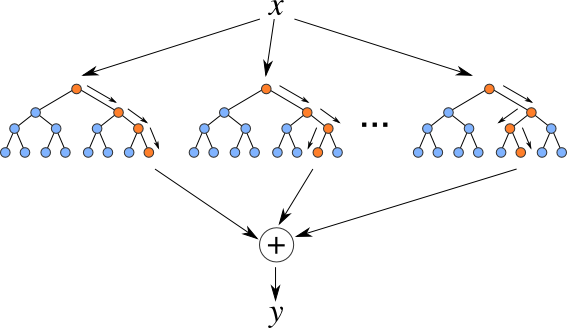
\includegraphics[scale=0.55]{monography/img/models/random_forest.png}
    \end{figure}
}

\slide{Support Vector Machine}{
    \begin{itemize}
        \item Não Paramétrico \& Supervisionado
        \item \(\epsilon\)-SVR 
        \item \(\abs{g(x) - f(x)} \leq \epsilon \)
        \item \textit{Kernel Trick}
    \end{itemize}
}

\slide{Support Vector Machine}{
    \begin{figure}[htbp]
        \centering
        \includegraphics[scale=0.55]{monography/img/models/svr_exemple.png}
    \end{figure}
}

\slide{Long Short-Term Memory}{
    \begin{itemize}
        \item Não Paramétrico \& Supervisionado
        \item Rede Neural Recorrente
        \item Conserta o sumiço do gradiente
        \item Utiliza de \textit{Gates} (entrada, saída e esquecimento) para controlar a informação que flui na rede
    \end{itemize}
}

\slide{Long Short-Term Memory}{
    \begin{figure}[htbp]
        \centering
        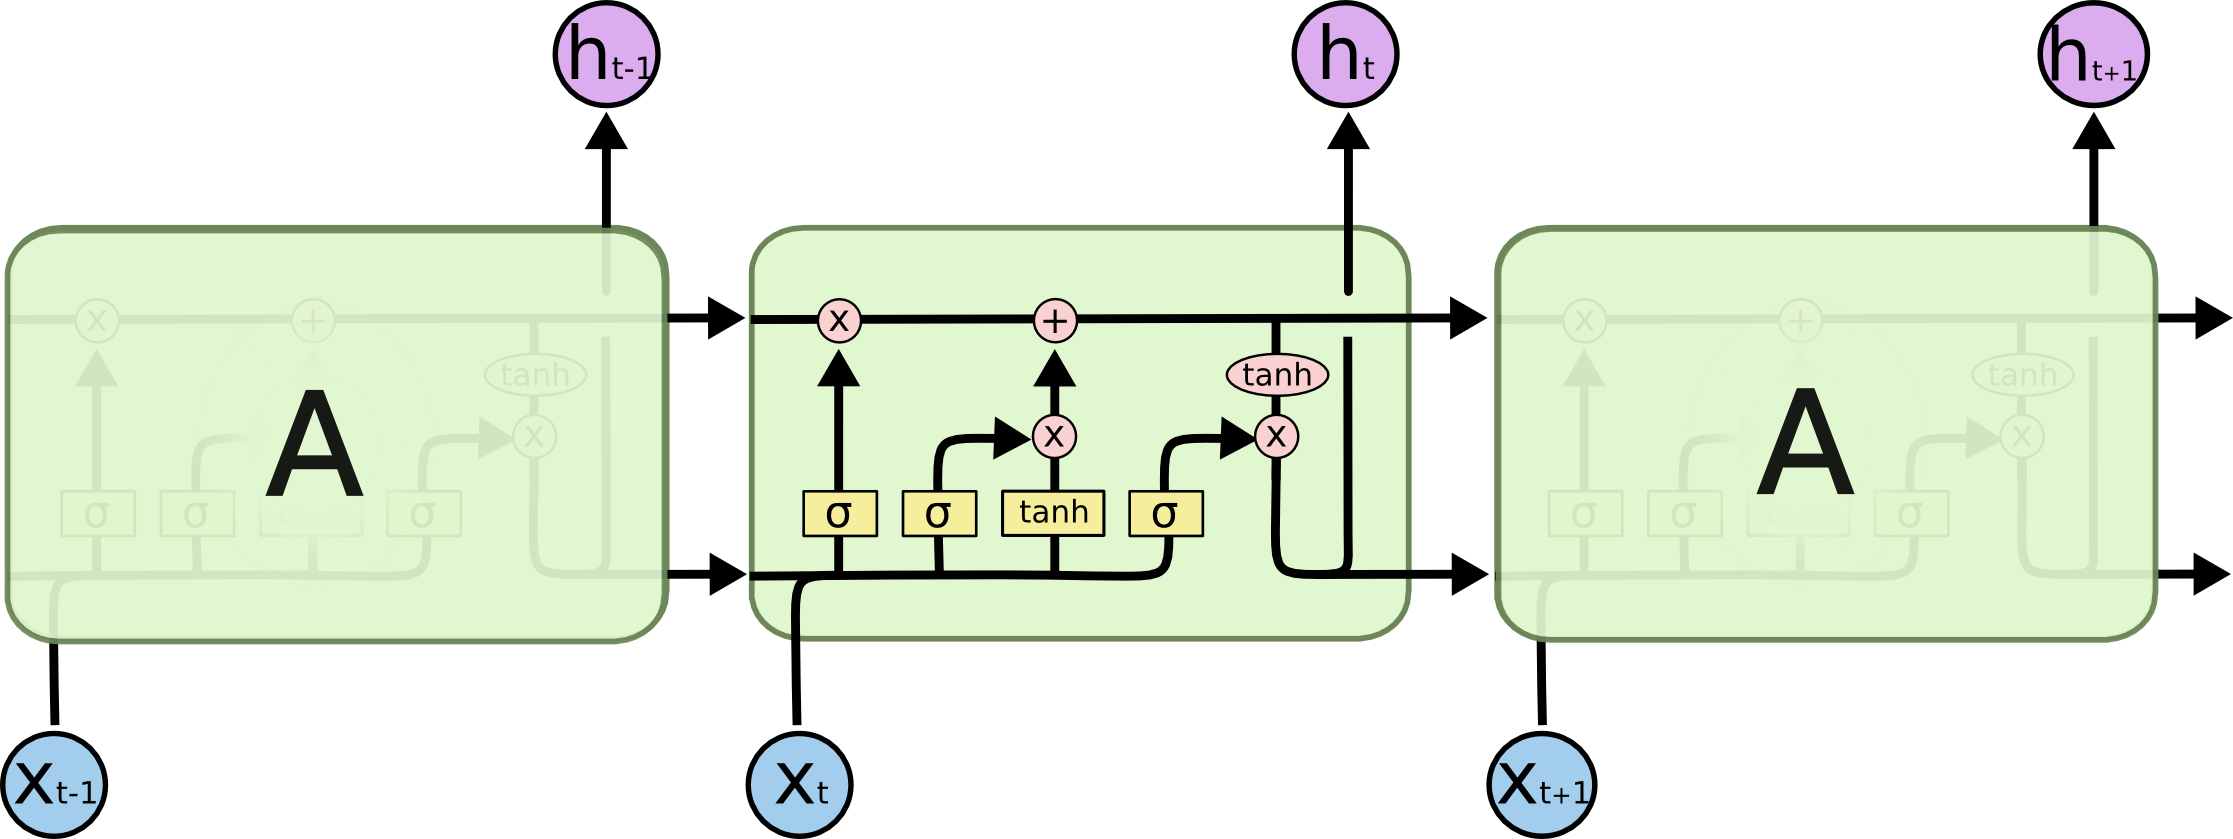
\includegraphics[scale=0.55]{monography/img/models/lstm3.png}
    \end{figure}
}

\slide{Gated Recurrent Unit}{
    \begin{itemize}
        \item Não Paramétrico \& Supervisionado
        \item Rede Neural Recorrente
        \item Similar a \textit{LSTM}, porém mais simples
        \item Utiliza de \textit{Gates} (entrada e atualização) para controlar a informação que flui na rede
    \end{itemize}
}

\slide{Gated Recurrent Unit}{
    \begin{figure}[htbp]
        \centering
        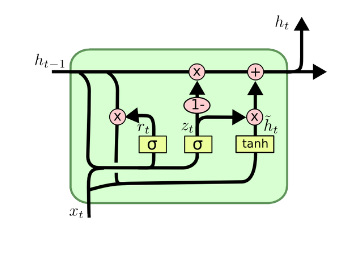
\includegraphics[scale=0.55]{monography/img/models/GRU.png}
    \end{figure}
}